\item \points{35} {\bf Semi-supervised EM}

\def\zsi{z^{(i)}}
\def\xsi{x^{(i)}}

Expectation Maximization (EM) is a classical algorithm for unsupervised learning (\emph{i.e.,} learning with hidden or latent variables). In this problem we will explore one of the ways in which EM algorithm can be adapted to the semi-supervised setting, where we have some labeled examples along with unlabeled examples.

In the standard unsupervised setting, we have $\nexp \in \mathbb{N}$ unlabeled examples $\{x^{(1)},\ldots,x^{(\nexp)}\}$. We wish to learn the parameters of $p(x,z;\theta)$ from the data, but $\zsi$'s are not observed. The classical EM algorithm is designed for this very purpose, where we maximize the intractable $p(x;\theta)$ indirectly by iteratively performing the E-step and M-step, each time maximizing a tractable lower bound of $p(x;\theta)$. Our objective can be concretely written as:

\begin{align*}
    \ell_{\text{unsup}}(\theta) &= \sum_{i=1}^\nexp \log p(\xsi;\theta) \\
    &= \sum_{i=1}^\nexp \log \sum_{\zsi} p(\xsi,\zsi;\theta)
\end{align*}


Now, we will attempt to construct an extension of EM to the semi-supervised setting. Let us suppose we have an \emph{additional} $\tilde{\nexp} \in \mathbb{N}$ labeled examples $\{(\tilde{x}^{(1)},\tilde{z}^{(1)}),\ldots,(\tilde{x}^{(\tilde{\nexp})},\tilde{z}^{(\tilde{\nexp})})\}$ where both $x$ and $z$ are observed. We want to simultaneously maximize the marginal likelihood of the parameters using the unlabeled examples, and full likelihood of the parameters using the labeled examples, by optimizing their weighted sum (with some hyperparameter $\alpha$). More concretely, our semi-supervised objective $\ell_\text{semi-sup}(\theta)$ can be written as:
%
\begin{align*}
    \ell_\text{sup}(\theta) &= \sum_{i=1}^{\tilde{\nexp}} \log p(\tilde{x}^{(i)},\tilde{z}^{(i)};\theta) \\
    \ell_{\text{semi-sup}}(\theta) &= \ell_\text{unsup}(\theta) + \alpha \ell_\text{sup}(\theta)
\end{align*}
%
We can derive the EM steps for the semi-supervised setting using the same approach and steps as before. You are \emph{strongly encouraged} to show to yourself (no need to include in the write-up) that we end up with:

\subsubsection*{E-step (semi-supervised)}

For each $i \in \{1,\ldots,\nexp\}$, set
\begin{align*}
    Q_i^{(t)}(\zsi) := p(\zsi|\xsi;\theta^{(t)})
\end{align*}

\subsubsection*{M-step (semi-supervised)}

\begin{align*}
    \theta^{(t+1)} &:= \arg\max_\theta\left[ \sum_{i=1}^\nexp\left( \sum_{\zsi} Q^{(t)}_i(\zsi) \log \frac{ p(\xsi, \zsi;\theta) }{ Q^{(t)}_i(\zsi)}\right)  + \alpha \left(\sum_{i=1}^{\tilde{\nexp}} \log p(\tilde{x}^{(i)},\tilde{z}^{(i)};\theta)\right)\right]
\end{align*}

\begin{enumerate}
  \item\subquestionpoints{5}
\textbf{Convergence.}
First we will show that this algorithm eventually converges. In order to prove this, it is sufficient to show that our semi-supervised objective $\ell_\text{semi-sup}(\theta)$ monotonically increases with each iteration of E and M step. Specifically, let $\theta^{(t)}$ be the parameters obtained at the end of $t$ EM-steps. Show that $\ell_\text{semi-sup}(\theta^{(t+1)}) \ge \ell_\text{semi-sup}(\theta^{(t)})$.


\ifnum\solutions=1 {
  \newcommand\tab[1][1cm]{\hspace*{#1}}
\begin{answer}
\\ \\
$l(\theta^{(t+1)}) = \alpha l_{sup}(\theta^{(t+1)}) +  l_{unsup}(\theta^{(t+1)})$ \\ \\
Jensen Equality \\ \\
\tab$\geq \  \alpha l_{sup}(\theta^{(t+1)}) +  \sum_{i=1}^n  \sum_{z^i} Q_i^t z^i log \frac{p(x^i,z^i;\theta^{t+1})}{Q_i^tz^i}$ \\ \\
\tab$\geq \  \alpha l_{sup}(\theta^{(t)}) +  \sum_{i=1}^n  \sum_{z^i} Q_i^t z^i log \frac{p(x^i,z^i;\theta^{t+1})}{p(z|x;\theta^t)}$ \\ \\
$\geq \alpha l_{sup}(\theta^{(t)}) +  l_{unsup}(\theta^{(t)})$\\ \\
$\geq  l(\theta^{(t)})$
\end{answer}

} \fi

\end{enumerate}


\subsubsection*{Semi-supervised GMM}
Now we will revisit the Gaussian Mixture Model (GMM), to apply our semi-supervised EM algorithm. Let us consider a scenario where data is generated from $k \in \mathbb{N}$ Gaussian distributions, with unknown means $\mu_j \in \R^\di$ and covariances $\Sigma_j \in \mathbb{S}_+^\di$ where $j \in \{1,\ldots,k\}$. We have $\nexp$ data points $\xsi \in \R^\di, i \in \{1,\ldots,\nexp\}$, and each data point has a corresponding latent (hidden/unknown) variable $\zsi \in \{1,\ldots,k\}$ indicating which distribution $\xsi$ belongs to. Specifically, $\zsi \sim \text{Multinomial}(\phi)$, such that $\sum_{j=1}^k\phi_j = 1$ and $\phi_j \ge 0$ for all $j$, and $\xsi|\zsi \sim \mathcal{N}\left(\mu_{\zsi}, \Sigma_{\zsi}\right)$ i.i.d. So, $\mu$, $\Sigma$, and $\phi$ are the model parameters.

We also have additional $\tilde{\nexp}$ data points $\tilde{x}^{(i)} \in \R^\di, i \in \{1,\ldots,\tilde{\nexp}\}$, and an associated \emph{observed} variable $\tilde{z}^{(i)} \in \{1,\ldots,k\}$ indicating the distribution $\tilde{x}^{(i)}$ belongs to. Note that $\tilde{z}^{(i)}$ are known constants (in contrast to $\zsi$ which are unknown \emph{random} variables). As before, we assume $\tilde{x}^{(i)}|\tilde{z}^{(i)} \sim \mathcal{N}\left(\mu_{\tilde{z}^{(i)}}, \Sigma_{\tilde{z}^{(i)}}\right)$ i.i.d.


In summary we have $\nexp$ + $\tilde{\nexp}$ examples, of which $\nexp$ are unlabeled data points $x$'s with unobserved $z$'s, and $\tilde{\nexp}$ are labeled data points $\tilde{x}^{(i)}$ with corresponding observed labels $\tilde{z}^{(i)}$. The traditional EM algorithm is designed to take only the $\nexp$ unlabeled examples as input, and learn the model parameters $\mu$, $\Sigma$, and $\phi$.


Our task now will be to apply the semi-supervised EM algorithm to GMMs in order to also leverage the additional $\tilde{\nexp}$ labeled examples, and come up with semi-supervised E-step and M-step update rules specific to GMMs. Whenever required, you can cite the lecture notes for derivations and steps.


\begin{enumerate}
  \setcounter{enumii}{1}
  \item\subquestionpoints{5} \textbf{Semi-supervised E-Step.}
Clearly state which are all the latent variables that need to be re-estimated in the E-step. Derive the E-step to re-estimate all the stated latent variables. Your final E-step expression must only involve $x, z, \mu, \Sigma, \phi$ and universal constants.


\ifnum\solutions=1 {
  \newcommand\tab[1][1cm]{\hspace*{#1}}
\begin{answer}
\\ \\
The latent variables are all the z(i), \\ \\
From the lecture notes: \\ \\
\tab$ w_j^i = Q_i(z^i = j ) = \frac{p(x^i|z^i=j;\mu,\sum)p(z^i = j)}{\sum_{l=1}^kp(x^i|z^i=l;\mu\sum)p(z^i=l)} $\\ \\
\tab[3cm]$ = \frac{  \frac{1}{ \sqrt{(2\pi)^d |\sum_j|}} exp( -\frac{1}{2} (x^i - \mu_j)^T \sum_j^{-1} (x^i - \mu_j)  )\phi_j } {\sum_{l=1}^k  \frac{1}{ \sqrt{(2\pi)^d |\sum_l|}} exp( -\frac{1}{2} (x^i - \mu_l)^T \sum_l^{-1} (x^i - \mu_l)  )\phi_j }$ \\ \\


\tab[3cm]$ = \frac{ |\sum_j|^{-\frac{1}{2}} exp( -\frac{1}{2} (x^i - \mu_j)^T \sum_j^{-1} (x^i - \mu_j)  )\phi_j } {\sum_{l=1}^k  |\sum_l|^{-\frac{1}{2}} exp( -\frac{1}{2} (x^i - \mu_l)^T \sum_l^{-1} (x^i - \mu_l)  )\phi_j }$ \\ \\


\end{answer}

} \fi

  \item\subquestionpoints{10} \textbf{Semi-supervised M-Step.}
Clearly state which are all the parameters that need to be re-estimated in the M-step. Derive the M-step to re-estimate all the stated parameters.  Specifically,
derive closed form expressions for the parameter update rules for $\mu^{(t+1)}$, $\Sigma^{(t+1)}$ and $\phi^{(t+1)}$ based on the semi-supervised objective.


\ifnum\solutions=1 {
  \begin{answer}
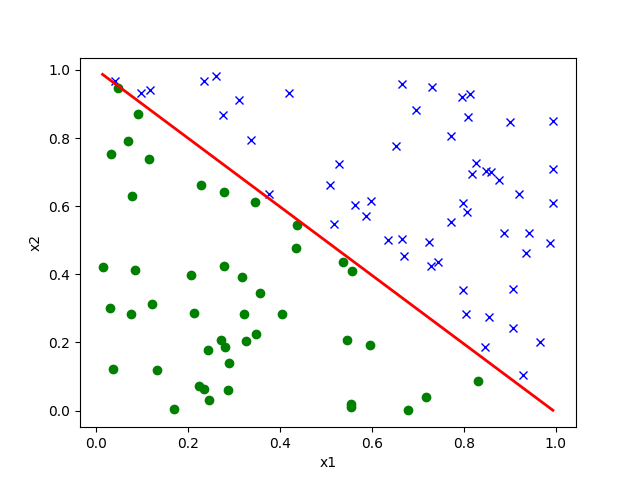
\includegraphics[width=15cm, height=20cm]{semi_supervised_em/1.png}
\includegraphics[width=15cm, height=20cm]{semi_supervised_em/2.png}
\end{answer}

} \fi


  \item\subquestionpoints{5} \textbf{Classical (Unsupervised) EM Implementation.}
For this sub-question, we are only going to consider the $\nexp$ unlabelled examples. Follow the instructions in \texttt{src/semi\_supervised\_em/gmm.py} to implement the traditional EM algorithm, and run it on the unlabelled data-set until convergence.

Run three trials and use the provided plotting function to construct a scatter plot of the resulting assignments to clusters (one plot for each trial). Your plot should indicate cluster assignments with colors they got assigned to (\emph{i.e.,} the cluster which had the highest probability in the final E-step).

\textbf{Submit the three plots obtained above in your write-up.}


\ifnum\solutions=1 {
  \begin{answer}
\begin{figure}[!h]
\minipage{0.32\textwidth}
  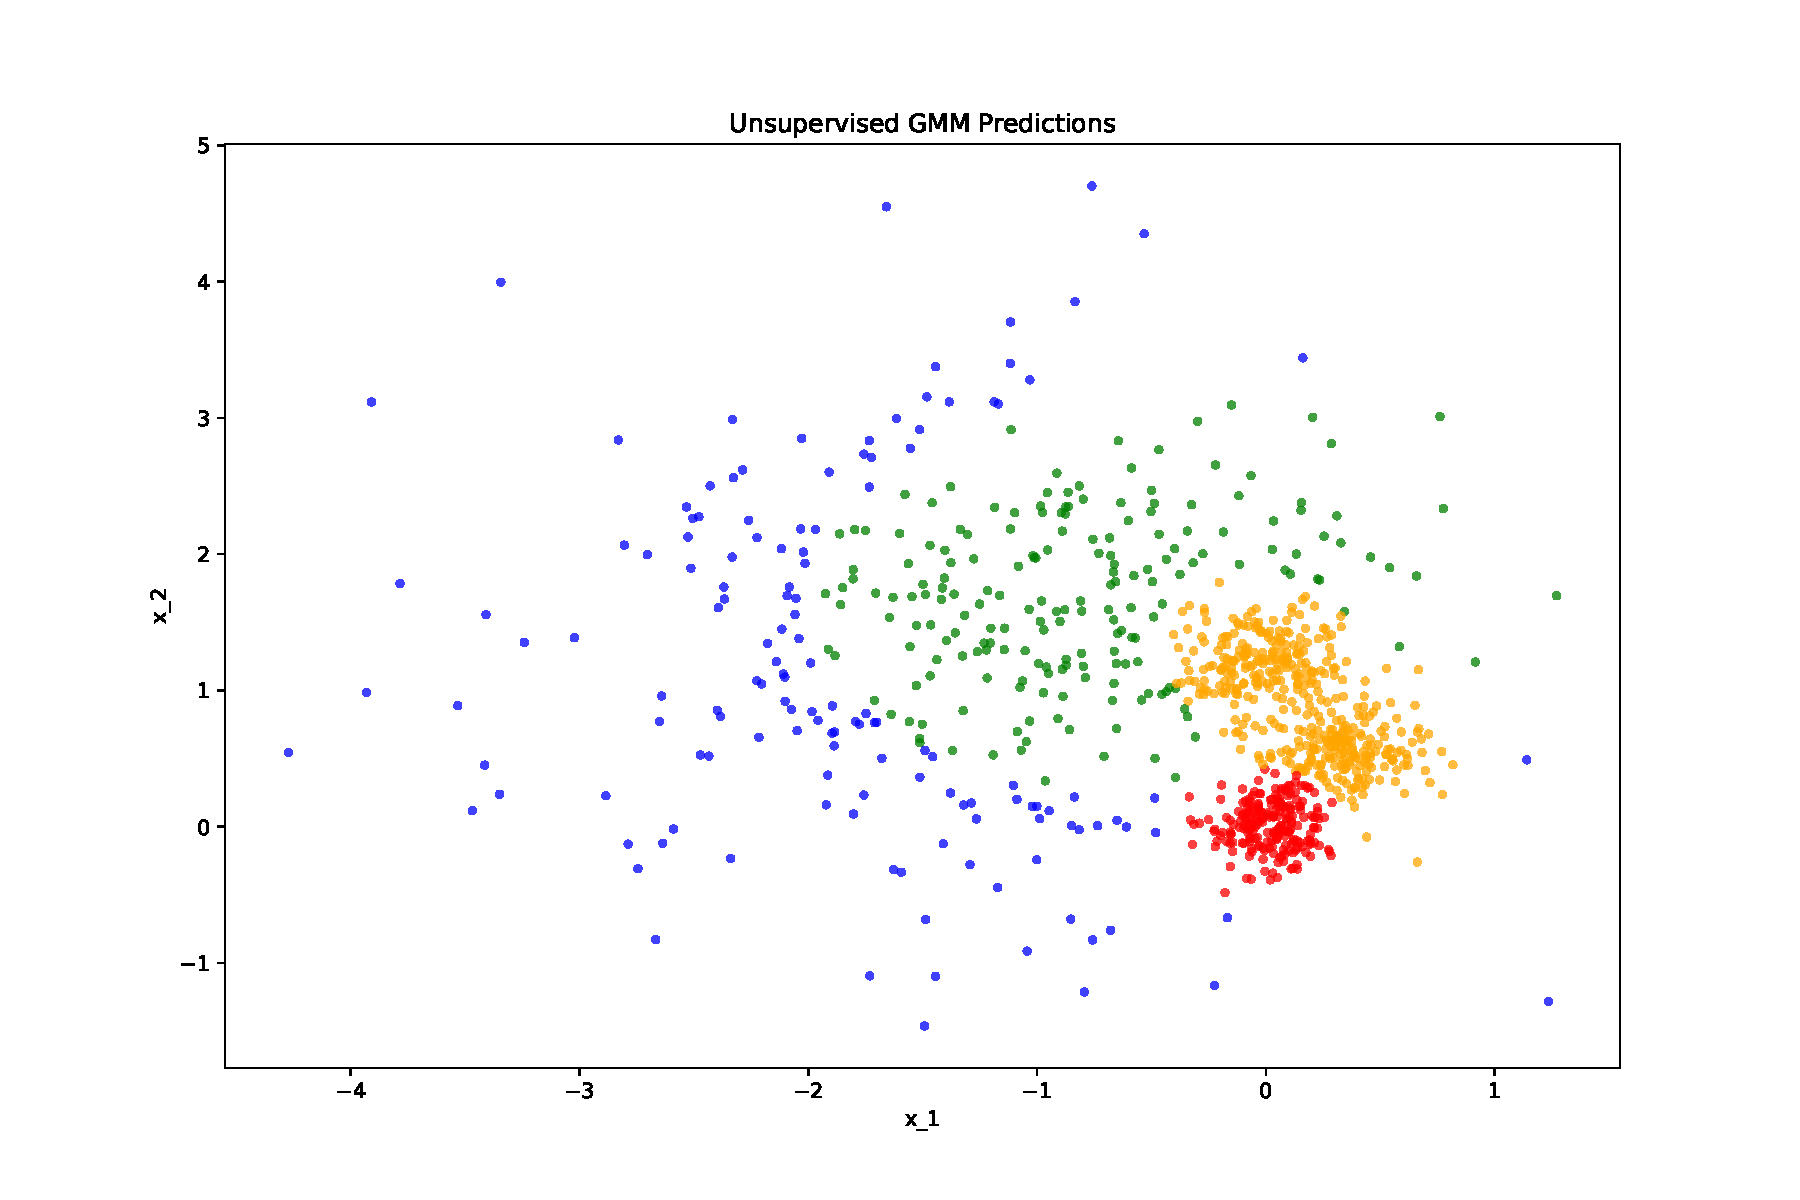
\includegraphics[width=\linewidth]{semi_supervised_em/pred_0.pdf}
\endminipage\hfill
\minipage{0.32\textwidth}
  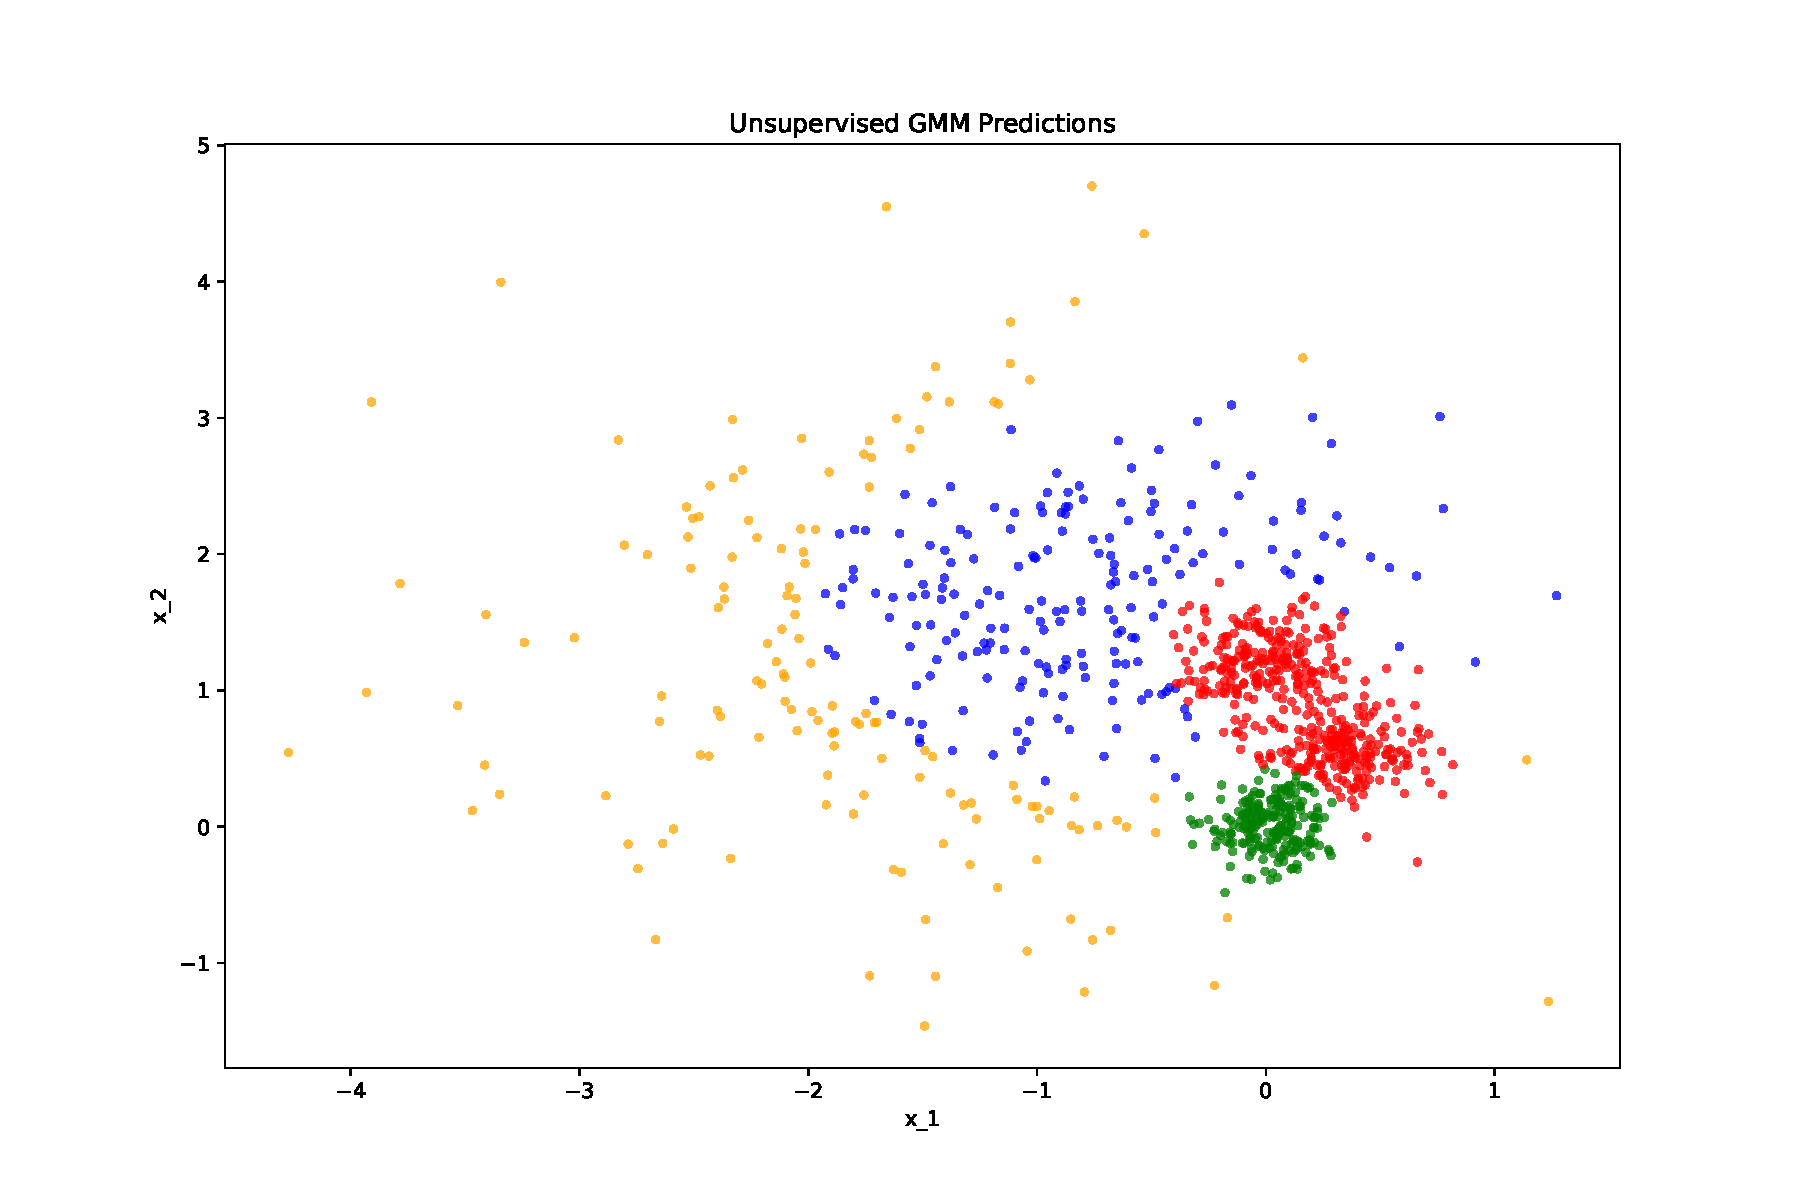
\includegraphics[width=\linewidth]{semi_supervised_em/pred_1.pdf}
\endminipage\hfill
\minipage{0.32\textwidth}%
  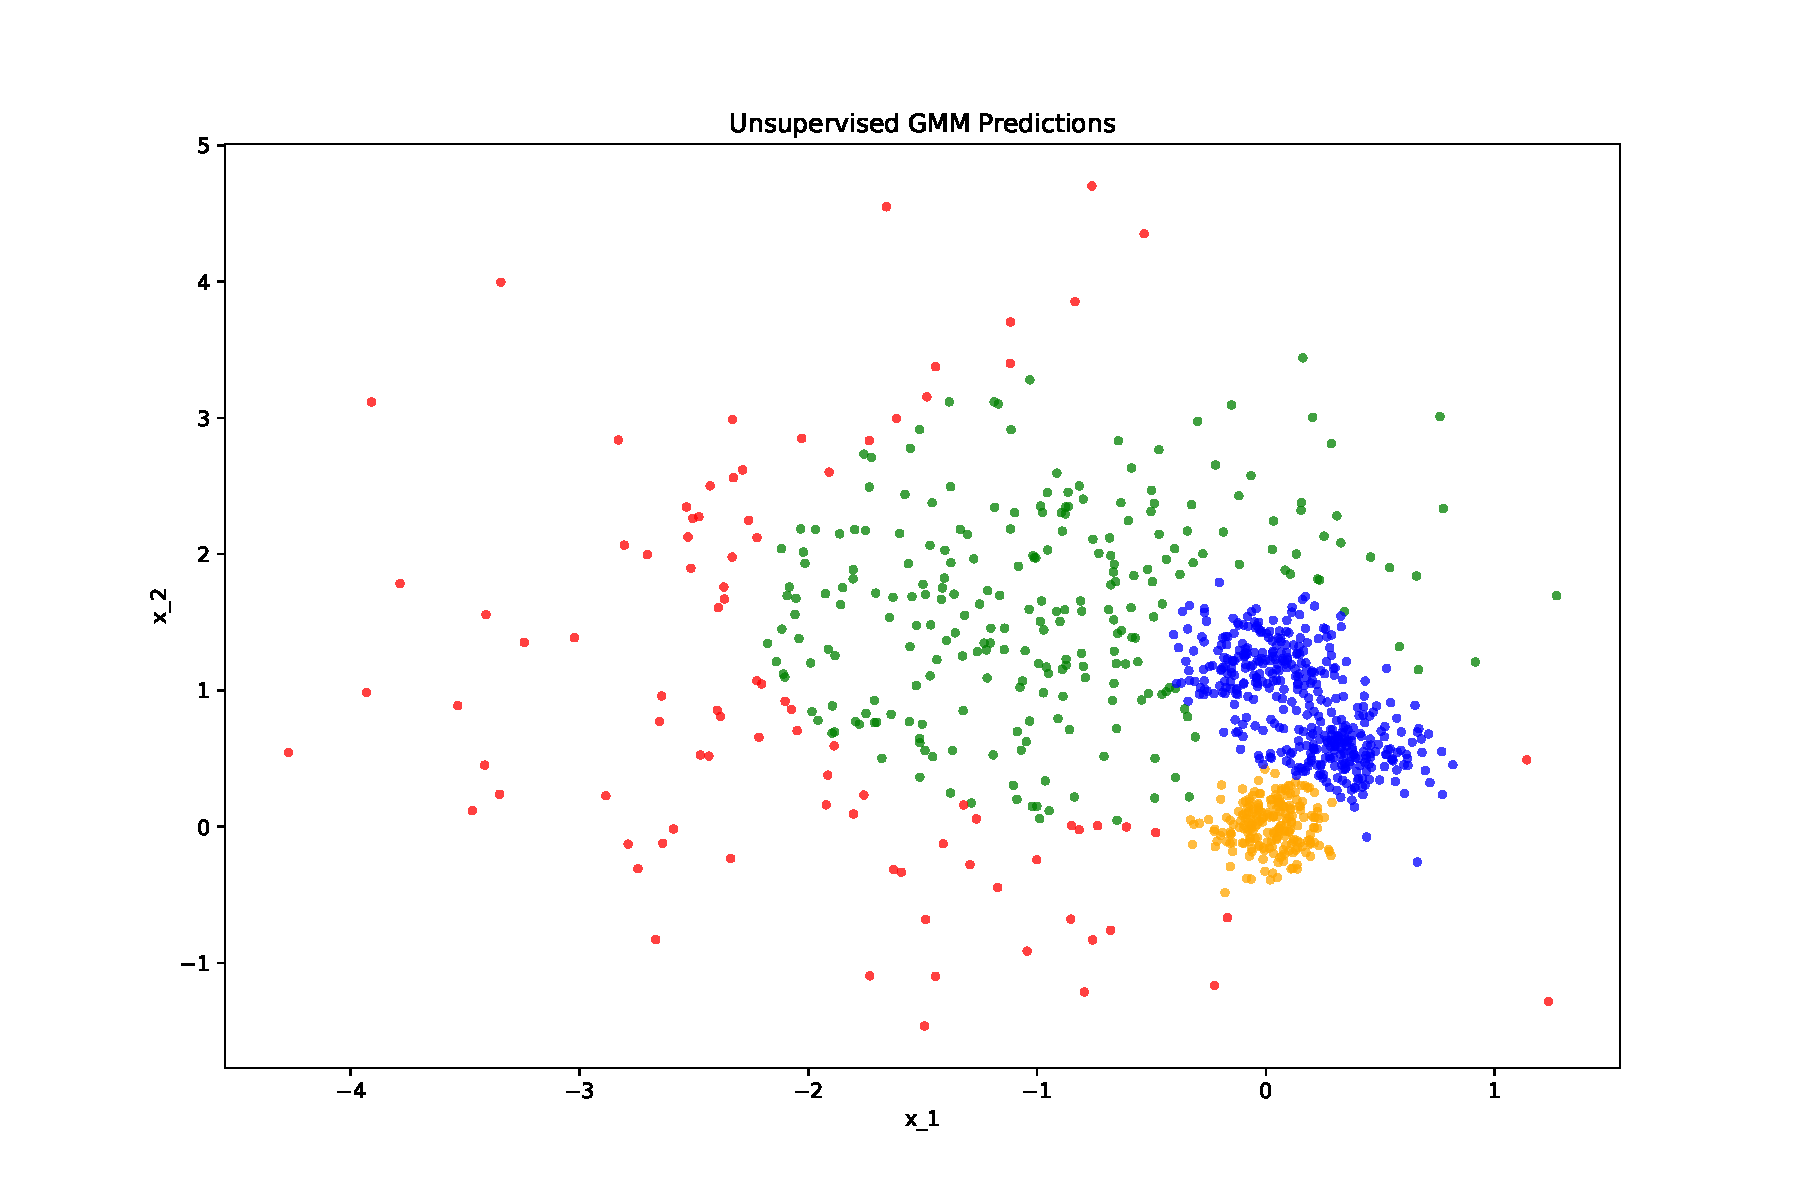
\includegraphics[width=\linewidth]{semi_supervised_em/pred_2.pdf}
\endminipage
\end{figure}
\\ \\  \\ \\ \\ \\ \\ \\ \\ \\ \\ \\ \\ \\ \\ \\ 
\end{answer}

} \fi

  \item\subquestionpoints{7} \textbf{Semi-supervised EM Implementation.}
Now we will consider both the labelled and unlabelled examples (a total of $\nexp + \tilde{\nexp}$), with 5 labelled examples per cluster. We have provided starter code for splitting the dataset into matrices \texttt{x} and \texttt{x\_tilde} of unlabelled and labelled examples respectively. Add to your code in \texttt{src/semi\_supervised\_em/gmm.py} to implement the modified EM algorithm, and run it on the dataset until convergence.

Create a plot for each trial, as done in the previous sub-question.

\textbf{Submit the three plots obtained above in your write-up.}


\ifnum\solutions=1 {
  \begin{answer}
\begin{figure}[!h]
\minipage{0.32\textwidth}
  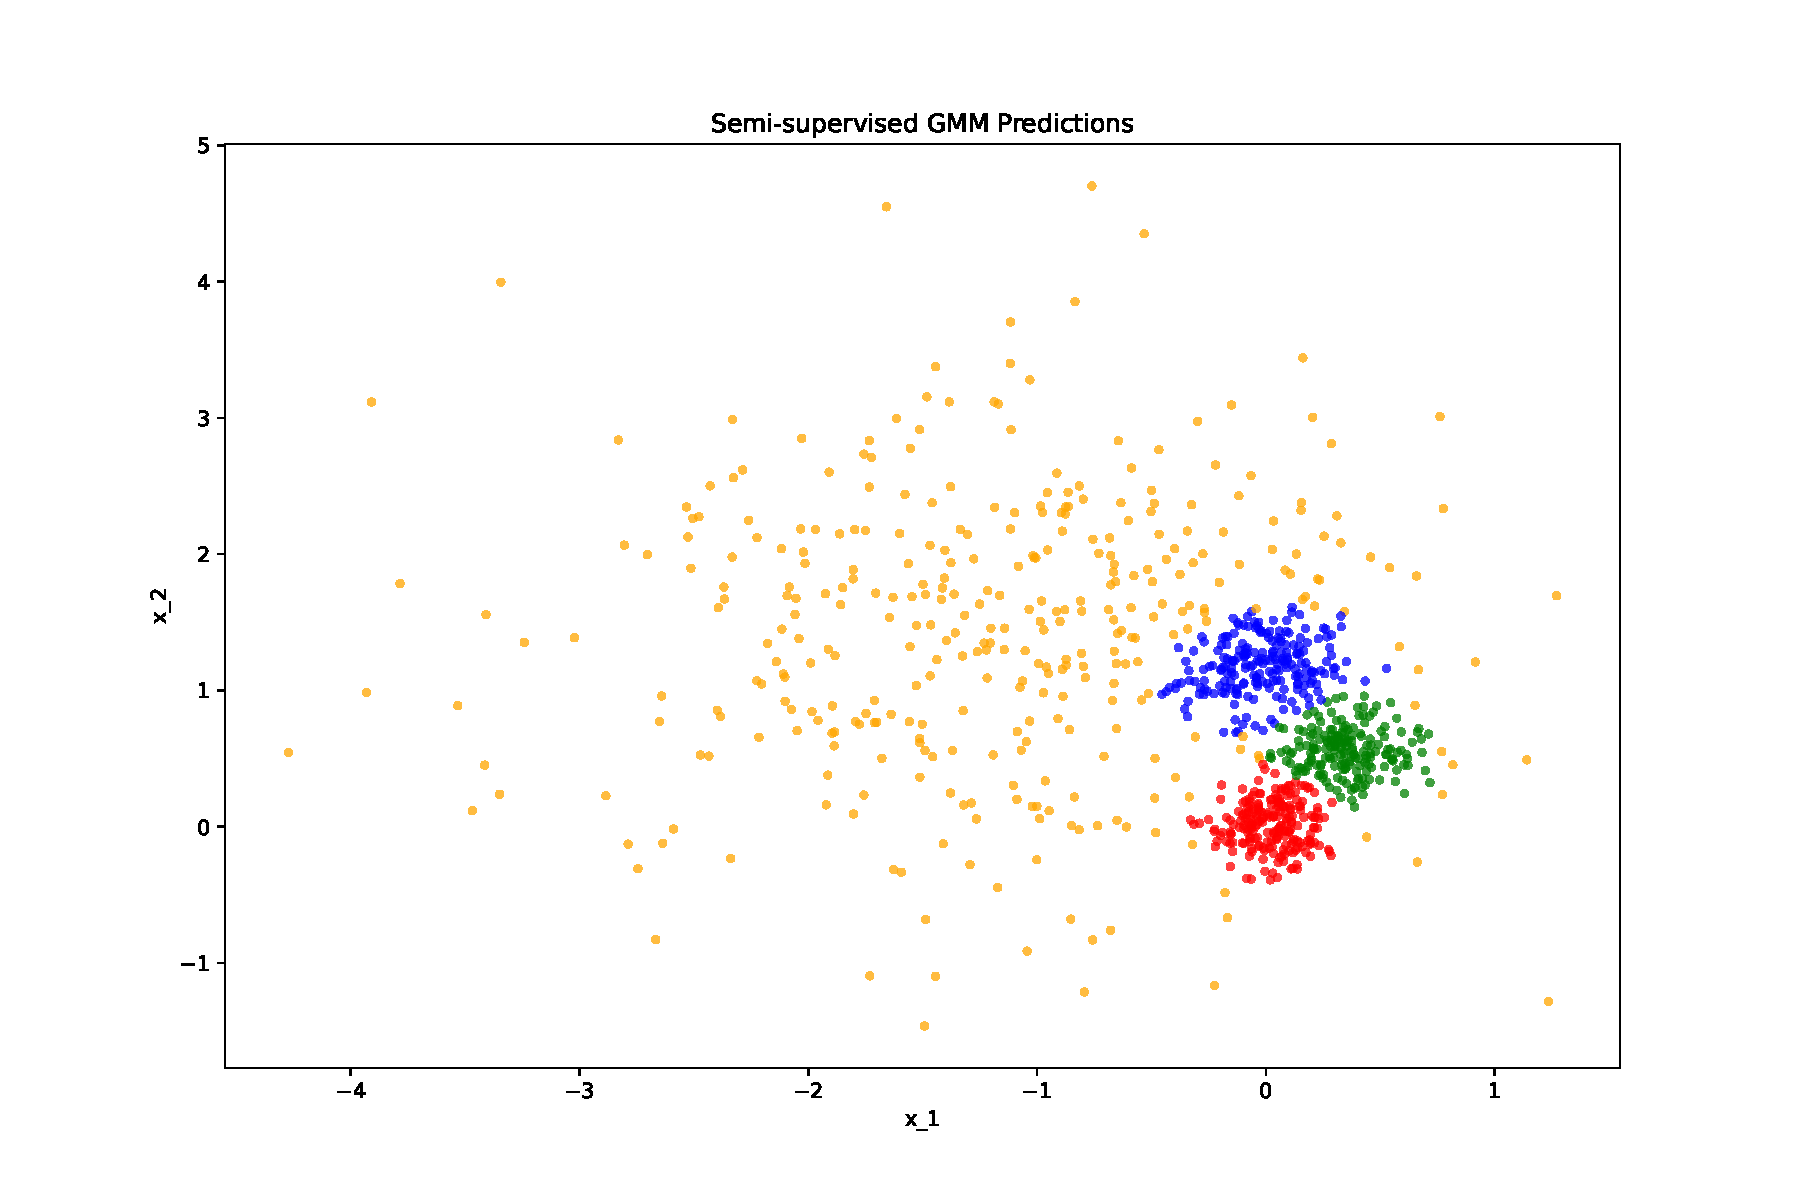
\includegraphics[width=\linewidth]{semi_supervised_em/pred_ss_0.pdf}
\endminipage\hfill
\minipage{0.32\textwidth}
  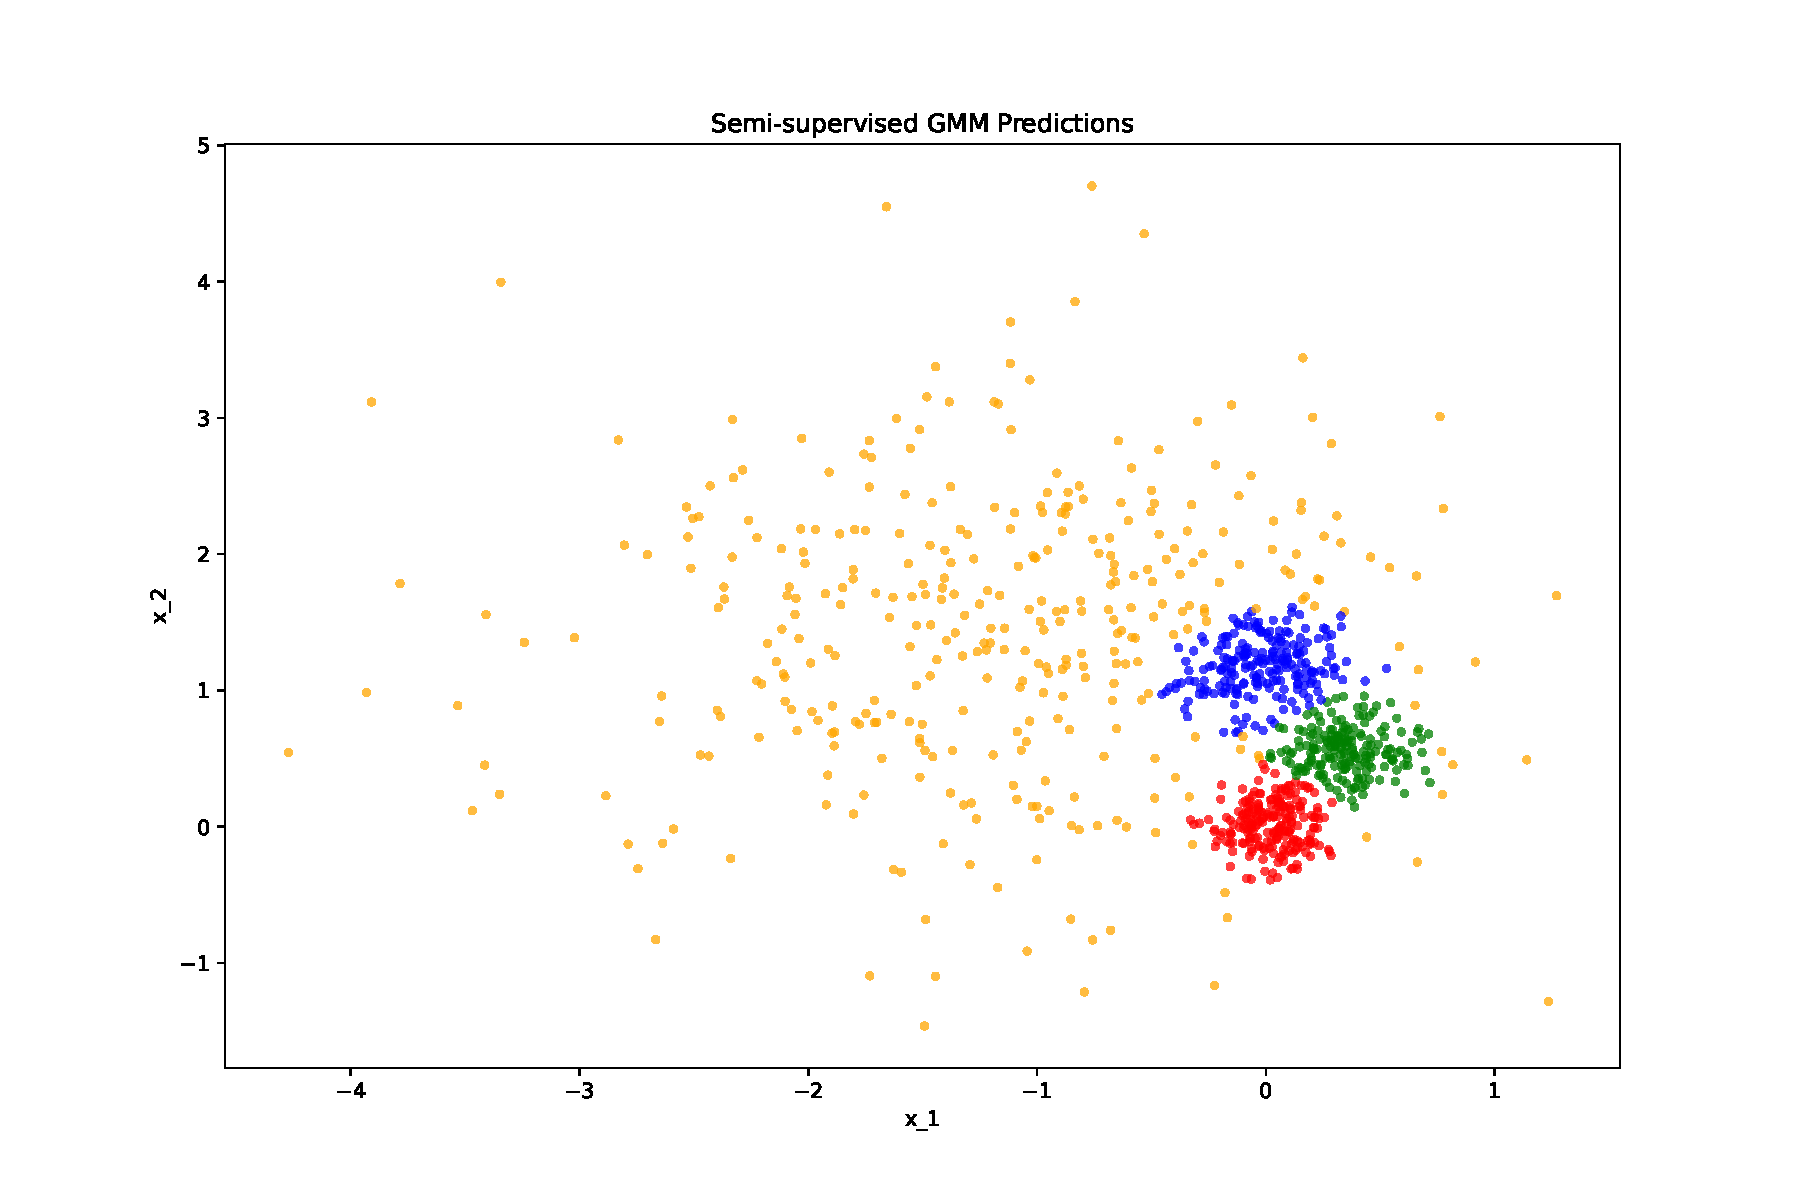
\includegraphics[width=\linewidth]{semi_supervised_em/pred_ss_1.pdf}
\endminipage\hfill
\minipage{0.32\textwidth}%
  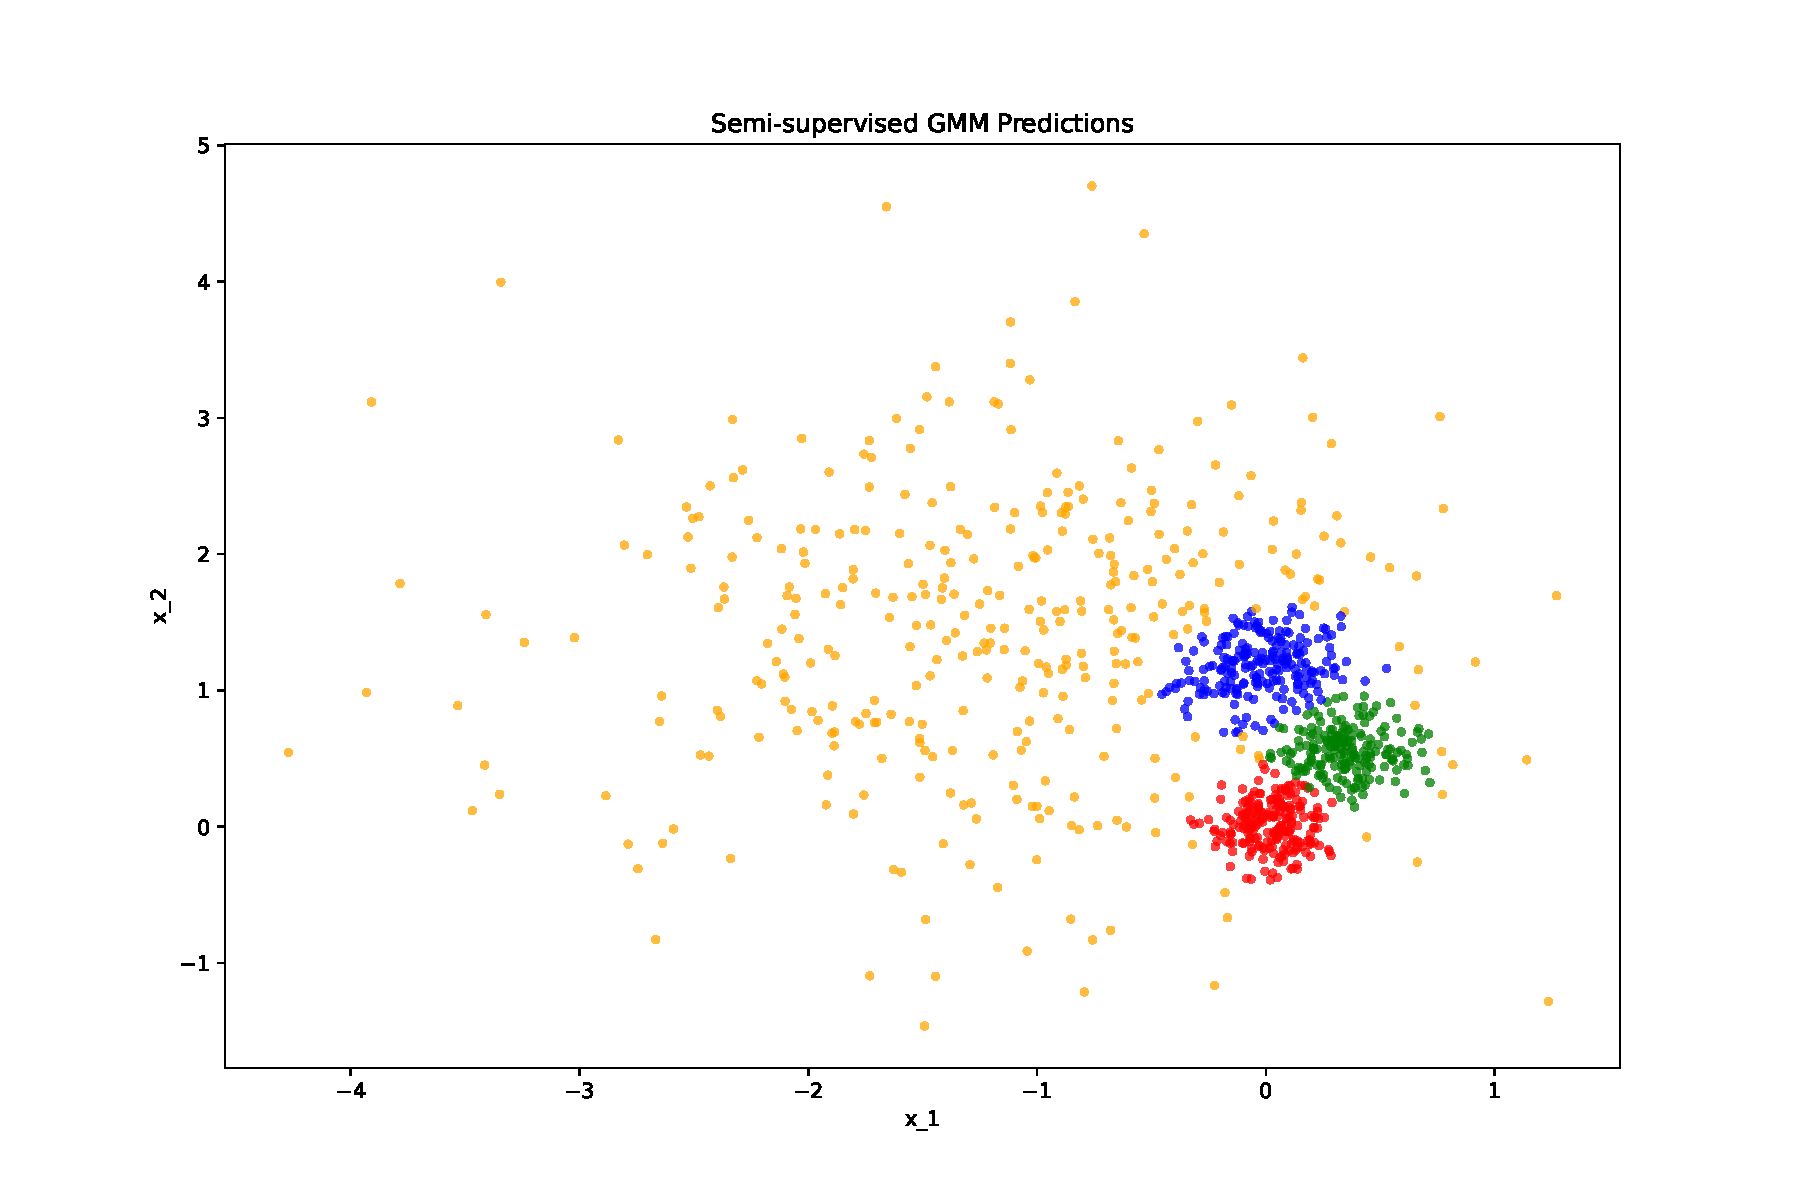
\includegraphics[width=\linewidth]{semi_supervised_em/pred_ss_2.pdf}
\endminipage
\end{figure}
\\ \\  \\ \\ \\ \\ \\ \\ \\ \\ \\ \\ \\ \\ \\ \\ 
\end{answer}

} \fi

  \item\subquestionpoints{3} \textbf{Comparison of Unsupervised and Semi-supervised EM.}
Briefly describe the differences you saw in unsupervised \emph{vs.} semi-supervised EM for each of the following:
\begin{enumerate}[label=\roman*.]
    \item Number of iterations taken to converge.
    \item Stability (\emph{i.e.,} how much did assignments change with different random initializations?)
    \item Overall quality of assignments.
\end{enumerate}

\textbf{Note:} The dataset was sampled from a mixture of three low-variance Gaussian distributions, and a fourth, high-variance Gaussian distribution. This should be useful in determining the overall quality of the assignments that were found by the two algorithms.


\ifnum\solutions=1 {
  \begin{answer}
\\ \\
Semi-supervised EM outperforms classical EM in all three categories, even with only 5 labeled instances per cluster. \\ \\
i. Unsupervised EM needs about 158 iterations to converge, whereas semi-supervised EM does so substantially faster. About 22 are needed for semi-supervised EM. \\ \\
ii. The stability of semi-supervised is substantially higher: In contrast to unsupervised learning, semi-supervised EM assignments are nearly identical. \\ \\
iii. The assignment is generally of higher quality when semi-supervised: Unsupervised EM has several different kinds of mistakes failing to discover there is just a single relatively high-variance Gaussian distribution in the mixture The underlying distribution is almost accurately revealed by semi-supervised EM. \\ \\
\end{answer}

} \fi

\end{enumerate}
